%\documentclass[12pt]{article}
\documentclass[12pt]{scrartcl}
\title{ELEC 340 Assignment 3}
\nonstopmode
%\usepackage[utf-8]{inputenc}
\usepackage{graphicx} % Required for including pictures
\usepackage[figurename=Figure]{caption}
\usepackage{float}    % For tables and other floats
\usepackage{verbatim} % For comments and other
\usepackage{amsmath}  % For math
\usepackage{amssymb}  % For more math
\usepackage{fullpage} % Set margins and place page numbers at bottom center
\usepackage{paralist} % paragraph spacing
\usepackage{listings} % For source code
\usepackage{subfig}   % For subfigures
%\usepackage{physics}  % for simplified dv, and 
\usepackage{enumitem} % useful for itemization
\usepackage{siunitx}  % standardization of si units

\usepackage[bitstream-charter]{mathdesign}
\usepackage[T1]{fontenc}

\usepackage{tikz,bm} % Useful for drawing plots
%\usepackage{tikz-3dplot}
\usepackage{circuitikz}
\usepackage[ruled,vlined]{algorithm2e}
\usepackage[utf8]{inputenc}
\usepackage{tikz}


%%% Colours used in field vectors and propagation direction
\definecolor{mycolor}{rgb}{1,0.2,0.3}
\definecolor{brightgreen}{rgb}{0.4, 1.0, 0.0}
\definecolor{britishracinggreen}{rgb}{0.0, 0.26, 0.15}
\definecolor{cadmiumgreen}{rgb}{0.0, 0.42, 0.24}
\definecolor{ceruleanblue}{rgb}{0.16, 0.32, 0.75}
\definecolor{darkelectricblue}{rgb}{0.33, 0.41, 0.47}
\definecolor{darkpowderblue}{rgb}{0.0, 0.2, 0.6}
\definecolor{darktangerine}{rgb}{1.0, 0.66, 0.07}
\definecolor{emerald}{rgb}{0.31, 0.78, 0.47}
\definecolor{palatinatepurple}{rgb}{0.41, 0.16, 0.38}
\definecolor{pastelviolet}{rgb}{0.8, 0.6, 0.79}

\usepackage{pdfpages}
\usepackage{graphicx}
\usepackage{float}

%---------- Listings config


\usepackage{color}

\definecolor{dkgreen}{rgb}{0,0.6,0}
\definecolor{gray}{rgb}{0.5,0.5,0.5}
\definecolor{mauve}{rgb}{0.58,0,0.82}

\lstset{frame=tb,
  language=Java,
  aboveskip=3mm,
  belowskip=3mm,
  showstringspaces=false,
  columns=flexible,
  basicstyle={\small\ttfamily},
  numbers=none,
  numberstyle=\tiny\color{gray},
  keywordstyle=\color{blue},
  commentstyle=\color{dkgreen},
  stringstyle=\color{mauve},
  breaklines=true,
  breakatwhitespace=true,
  tabsize=3
}



\begin{document}

\begin{center}
	\hrule
	\vspace{.4cm}
	{\textbf { \large \scshape{ Práctica 1 - Regresión lineal y gradiente descendente}}}
\end{center}
{\ Javier Sáez \hspace{\fill} Aprendizaje Automático  \\
	\hrule


\subsection*{Nota previa}

Se declara en la práctica una función \lstinline{to_numpy(func)}, que nos servirá de ayuda para la implementación. El código es muy sencillo:

\begin{lstlisting}[language=Python]
  def to_numpy(func):
  """Decorador para convertir funciones a versión NumPy"""
  def numpy_func(w):
    return func(*w)

  return numpy_func
\end{lstlisting}
Esta nos será de gran utilidad a la hora de evaluar funciones en puntos concretos. Si una función toma dos parámetros, $x_1$ y $x_2$, nos permite pasarle un único parámetro que sea un vector con dos posiciones.
Por ejemplo, si $f: \mathbb R^2 \to \mathbb R$, en lugar de tener que hacer $f(a,b)$, podemos hacer simplemente $f(c)$ en nuestro código, donde $c$ será un vector $c = [c_1,c_2]$.

\section*{Ejercicio 1}

En este ejercicio, se implementará el algoritmo de descenso de gradiente (o gradiente descendente) y se aplicará
este sobre varias funciones con el objetivo de estudiar cómo afecta tanto el punto inicial 
como la tasa de aprendizaje $\eta$ a la solución que este algoritmo encuentra.\\

Lo primero que debemos hacer es recordar en qué consiste el algoritmo de descenso de gradiente,
 veámoslo en pseudocódigo:\\


\begin{algorithm}[H]
\SetAlgoLined
\KwResult{Mínimo local de una función}
 parametros: $\eta$, $f$, $max\_iteraciones$,$criterio\_parada$, $punto\_inicial$ \;

 $punto  \leftarrow punto\_inicial$ \;
 \While{No (Criterio de parada)}{
     $gradiente \leftarrow \nabla f(punto)$ \;
     $direccion \leftarrow - gradiente$ \;
     $punto \leftarrow punto - \eta \cdot direccion$
 }
 \caption{Descenso de gradiente}
\end{algorithm}

En la implementación en el lenguaje de programación escogido, \emph{python}, se podrá hacer todo el contenido de este bucle while en una única línea.
Sin embargo, se añadirá contenido extra al cuerpo de la función para que nos devuelva no solo el mínimo, sino también toda la sucesión de puntos
que se han ido obteniendo así como el número de iteraciones que se han dado. En este caso, consideraremos una iteración claramente como una actualización del punto mínimo
de la función. \\

\begin{lstlisting}[language=Python]
    def gradient_descent(eta,fun,grad_fun,maxIter,error2get,initial_point):
	    iterations = 0
	    w_t = initial_point
	    all_w = []
	    all_w.append(w_t)

	    while iterations < maxIter and fun(w_t) > error2get:
		    # All gradient descent in 1 line
		    w_t = w_t - eta*grad_fun(w_t)
		    all_w.append(w_t)
		    iterations += 1
	

	    return np.array(all_w),w_t, iterations
\end{lstlisting}


\subsection*{Apartado 2}
Consideremos ahora la función

$$
E(u,v) = \left( u^3 e^{(v-2)} - 2v^2 e^{-u}\right)^2.
$$


Nuestra función $E$ es claramente derivable , así que procedemos a obtener sus derivadas parciales para poder aplicarle el algoritmo. Obtenemos que
$$
\frac{\partial E}{\partial u} = 2 \left( u^3 e^{(v-2)} - 2v^2 e^{-u}\right)\left( 3u^2 e^{(v-2)} + 2v^2 e^{-u}\right)
$$
y
$$
\frac{\partial E}{\partial v} = 2 \left( u^3 e^{(v-2)} - 2v^2 e^{-u}\right) \left( u^3 e^{(v-2)} - 4v e^{-u}\right).
$$

Tras definir una función para cada una de estas derivadas parciales y una para darnos el gradiente $\nabla E = \left(\frac{\partial E}{\partial u}, \frac{\partial E}{\partial v}\right)$ de $E$ en un punto
, podemos aplicar el algoritmo. Los parámetros de la ejecución son los siguientes:
\begin{itemize}
\item Tasa de aprendizaje $\eta = 0.1$.
\item Punto inicial $(u,v) = (1,1)$.
\item Condición de parada: Error $E$ inferior a $10^{-14}$ (esto está programado directamente en la función).
\item Máximo de iteraciones: prácticamente ilimitado ($10.000.000.000$) para este primer ejercicio.
\end{itemize}

Tras la obtención del gráfico, se ha programado también una pequeña función que formatea la salida de algunos datos que pueden ser relevantes.
En particular, dada la propia función en un string, los parámetros del gradiente descendente y los resultados obtenidos del mismo,
esta función imprimirá estos parámetros, y los resultados obtenidos entre ellos el número de iteraciones y el punto final. Esta función se llama \lstinline{print_output_e1}
y el resultado sobre este problema es:

\begin{lstlisting}[language=bash]
    Gradiente descendente sobre la función: E(u,v) = (u^3 e^(v-2) - 2v^2 e^(-u))^2
    Punto inicial: [1. 1.]
    Tasa de aprendizaje: 0.1
    Numero de iteraciones:  10
    Coordenadas obtenidas: ( 1.1572888496465497 ,  0.9108383657484799 )
    Valor de la función de error en el mínimo :  3.1139605842768533e-15
\end{lstlisting}

Donde podemos ver las \textbf{iteraciones} que tarda el algoritmo en obtener por primera vez un valor de $E(u,v)$ por debajo de lo pedido, y además también
se observan las \textbf{coordenadas} en las que esto ocurre. Veamos cuál es la salida de dibujar la función y el mínimo por pantalla:

\begin{figure}[H]
  \centering
  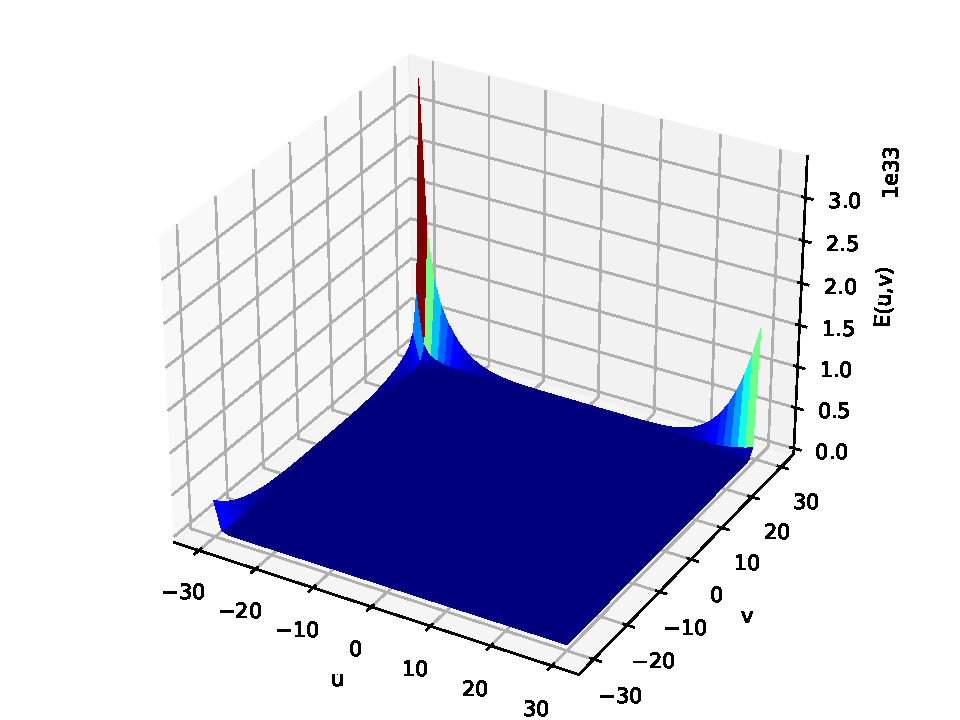
\includegraphics[scale=0.6]{media/E1-1.pdf}
  \caption{Mínimo local de la función}
\end{figure}

En este caso, el símbolo de estrella que simboliza el mínimo es muy difícilmente visible en el centro de la imagen. Esto es debido al rango dado para los ejes por defecto en el dibujo.
Vamos a dibujar ahora todos los puntos que ha ido obteniendo el algoritmo de descenso por el gradiente (para esto hemos devuelto una variable más en el código de la función) para ver cómo se ha ido buscando 
el mínimo de la función. El resultado es el siguiente:

\begin{figure}[H]
  \centering
  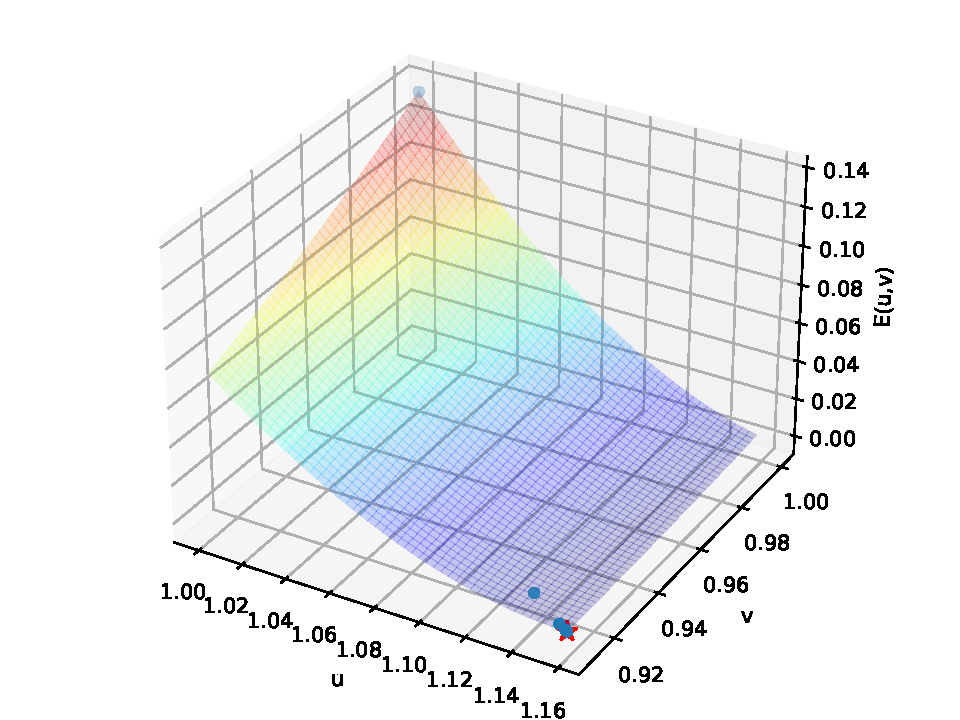
\includegraphics[scale=0.6]{media/E1-1-all.pdf}
  \caption{Mirada cercana al mínimo de la función}
\end{figure}

En esta imagen, obtenida usando el mismo código que la anterior salvo que el rango de dibujado de la superficie es únicamente el máximo de las coordenadas de los puntos que ha ido
obteniendo el algoritmo, se puede observar mucho mejor que se encuentra un mínimo local y como las iteraciones van buscando ese mínimo.

Se puede además observar usando la función \lstinline{plot_fun_evolution} cómo evoluciona el valor 
de la función $E(u,v)$ con las iteraciones. El resultado es el siguiente:

\begin{figure}[H]
  \centering
  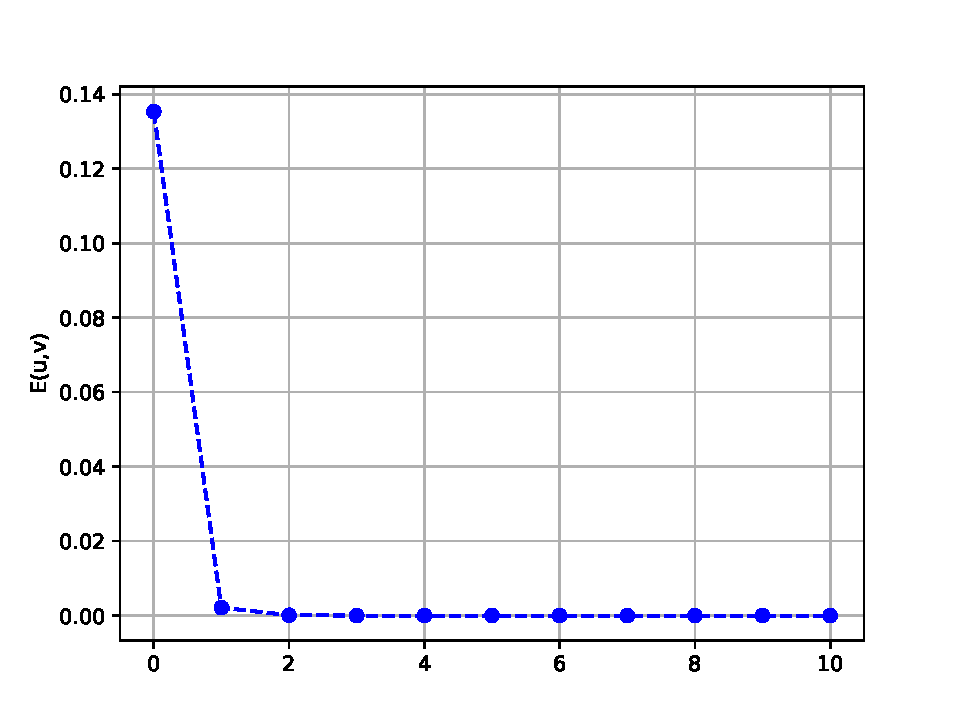
\includegraphics[scale=0.6]{media/f_evolution_e1-1.pdf}
  \caption{Valor de $E(u,v)$ en cada iteración.}
\end{figure}

Como vemos, el valor del error desciende en apenas dos iteraciones hasta muy cerca del mínimo y en las siguientes al estar posiblemente cerca de un mínimo no hay mucha variación en la función y se sigue iterando hasta que el valor esté
por debajo del deseado.

\subsection*{Apartado 3}

Vamos a considerar ahora una nueva función. Consideramos $f: \mathbb R^2 \to \mathbb R$ dada por:
\begin{equation}\label{eq:f}
f(x,y) = (x+2)^2 + 2(y-2)^2 + 2\sin(2\pi x) \sin(2\pi y). 
\end{equation}
Por ser suma y producto de funciones derivables, es de nuevo una función derivable, cuyo gradiente viene dado por:
$$
\nabla f(x,y) = \Big( 2(x+2)  +4 \pi \cos(2 \pi x ) \sin (2 \pi y),\ 4 (y-2) + 4\pi \sin(2 \pi x) \cos (2 \pi y)\Big)
$$

La implementación de esta función en \emph{python} es la siguiente:\\

\begin{lstlisting}[language=Python]
  def f(x,y):
	  return (x + 2)**2 + 2*(y - 2)**2 + 2 * np.sin(2 * np.pi * x) * np.sin(2 * np.pi * y)

  def dfx(x,y):
	  return 2 * (x+2) + 4 * np.pi * np.cos(2* np.pi * x) * np.sin(2* np.pi * y)

  def dfy(x,y):
	  return 4 * (y-2) + 4 * np.pi * np.sin(2 * np.pi * x) * np.cos(2 * np.pi * y) 
\end{lstlisting}


Todas estas funciones en el código llevan el decorador \lstinline{@to_numpy} para poder llamarlas con un solo parámetro. Una vez implementado, volvemos a ejecutar el algoritmo de descenso según el gradiente en esta función. Esta vez, los parámetros son los siguientes:
\begin{itemize}
\item Punto inicial $(-1,1)$.
\item Tasa de aprendizaje $\eta = 0.01$.
\item Máximo de iteraciones $50$.
\item En este caso, suprimimos la condición del error a obtener, simplemente indicando que el error sea \lstinline{-math.inf}, y que se
realicen así las $50$ iteraciones.
\end{itemize}

El resultado de la ejecución es el siguiente:

\begin{lstlisting}[language=bash]
Gradiente descendente sobre la función: f(x,y) = (x+2)^2 + 2(y-2)^2 + 2 sin(2pi x) sin(2pi y)
Punto inicial: [-1.  1.]
Tasa de aprendizaje: 0.01
Numero de iteraciones:  50
Coordenadas obtenidas: ( -1.269064351751895 ,  1.2867208738332965 )
Valor de la función de error en el mínimo :  -0.3812494974381
\end{lstlisting}

Podemos ver el gráfico que nos genera la función utilizada en el ejercicio anterior para ver cómo desciende el valor de la función con las iteraciones.

\begin{figure}[H]
  \centering
  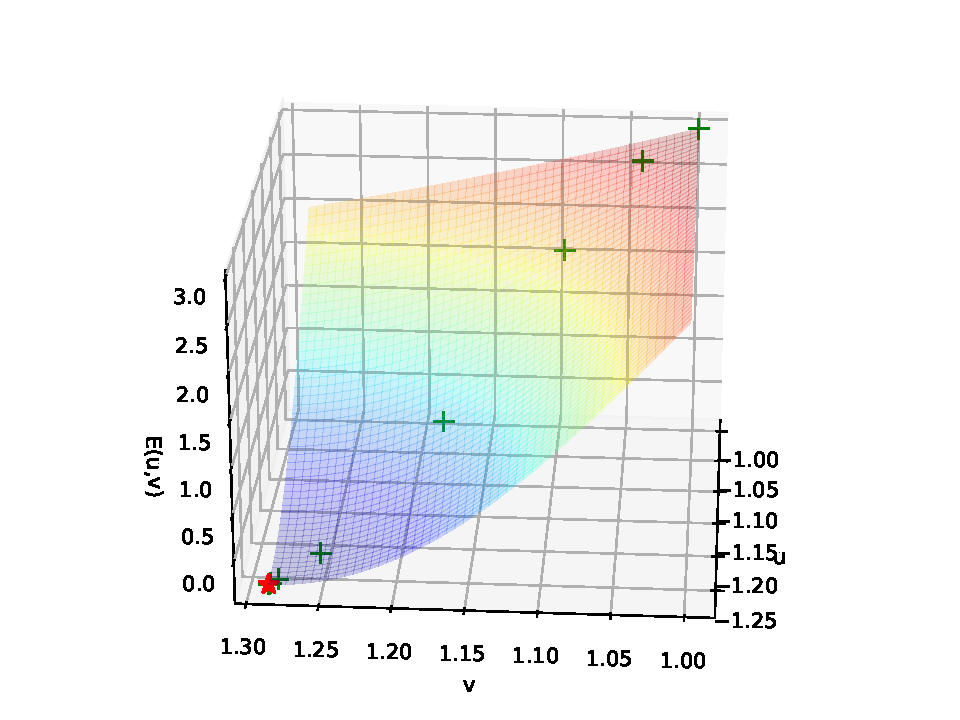
\includegraphics[scale=0.6]{media/E1-2-all-moved.pdf}
  \caption{Iteraciones en búsqueda del mínimo en $f(x,y)$ con $\eta = 0.01$.}
\end{figure}

Vemos como, igual que en el caso anterior, se encuentra el mínimo local en pocas iteraciones. Podemos ver cómo ha descendido la función según las iteraciones:

\begin{figure}[H]
  \centering
  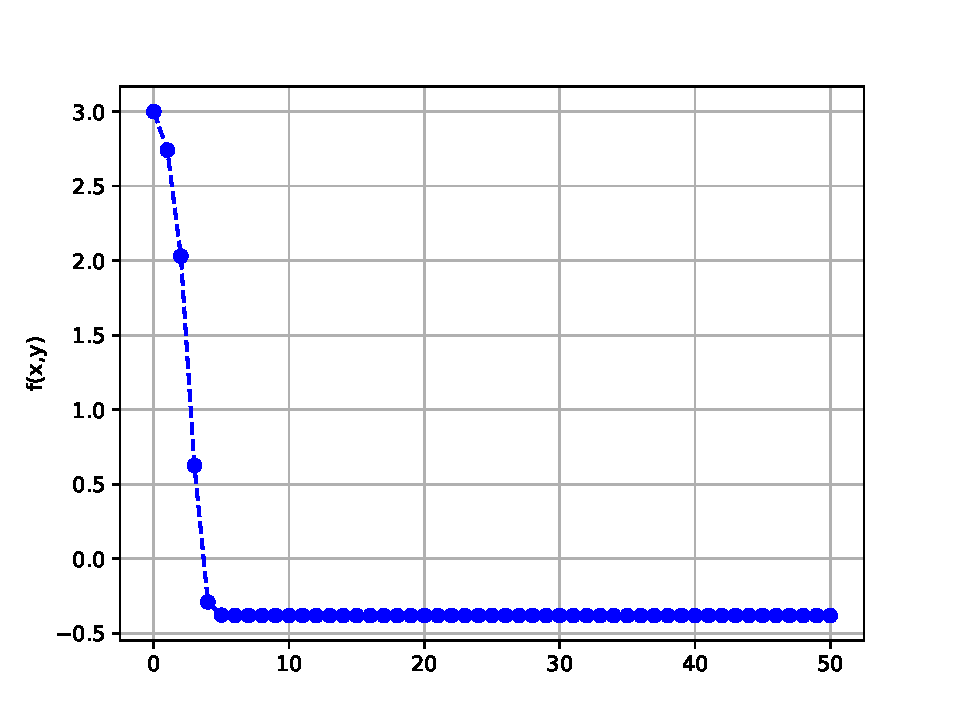
\includegraphics[scale=0.6]{media/f_evolution_e1-2-001.pdf}
  \caption{Valor de $f(x,y)$ en cada iteración con $\eta = 0.01$.}
\end{figure}

Podemos ver cómo se estabiliza rápidamente (unas $4$ iteraciones) y luego se mantiene en un error muy similar gracias al pequeño valor de $\eta$.

Vamos a volver a repetir el experimento pero ahora usando $\eta = 0.1$, lo cual supone un cambio bastante grande. El resultado es el siguiente:

\begin{lstlisting}[language=bash]
Gradiente descendente sobre la función: f(x,y) = (x+2)^2 + 2(y-2)^2 + 2 sin(2pi x) sin(2pi y)
Punto inicial: [-1.  1.]
Tasa de aprendizaje: 0.1
Numero de iteraciones:  50
Coordenadas obtenidas: ( -2.9604132205400098 ,  0.5733549488050332 )
Valor de la función de error en el mínimo :  4.774050376444264
\end{lstlisting}

Se puede ya observar como el valor encontrado esta vez es muy diferente, además de ser claramente superior en su valor de $f$. 
Esto es debido a que al ser la tasa de aprendizaje $\eta$ mucho mayor, los saltos que se dan en la dirección opuesta a la del gradiente son de gran tamaño y se salta en la función a sitios en los que los mínimos son
diferentes que en el punto inicial, y el gradiente puede tener además una dirección completamente diferente a la que tenía en el punto anterior, por lo que la dirección de la nueva iteración puede cambiar mucho de nuevo. Vemos el resultado de todos los saltos que
da el algoritmo de descenso según el gradiente:

\begin{figure}[H]
  \centering
  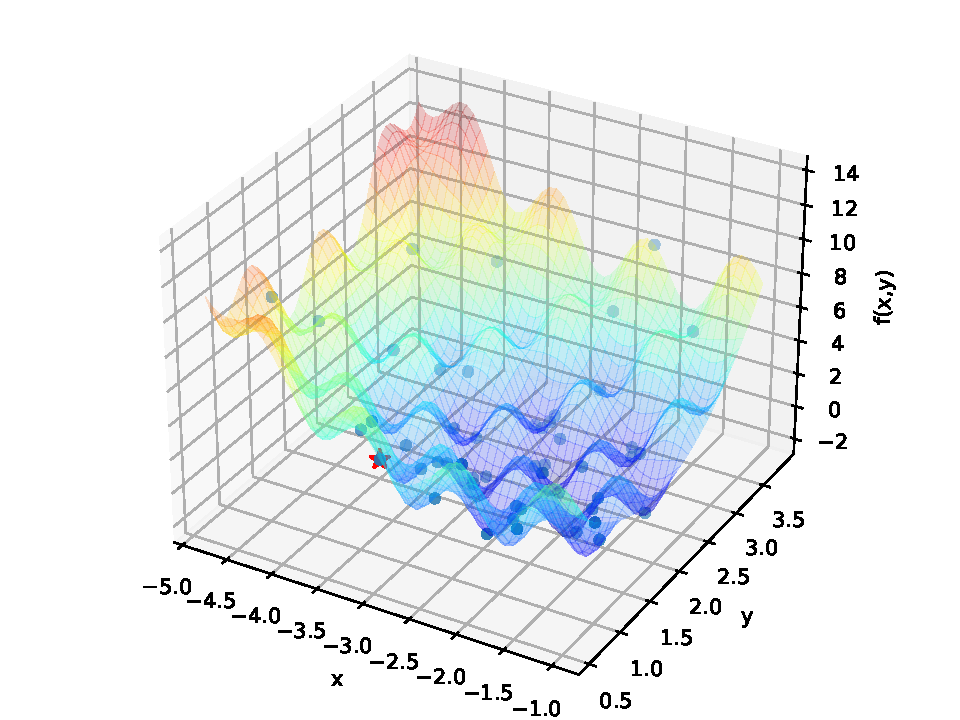
\includegraphics[scale=0.6]{media/E1-2-loweta-all.pdf}
  \caption{Iteraciones en búsqueda del mínimo en $f(x,y)$ con $\eta = 0.1$.}
\end{figure}

De hecho, si nos fijamos en qué valores toma la función en las iteraciones, vemos que no se estabiliza al ser el $\eta$ tan grande:

\begin{figure}[H]
  \centering
  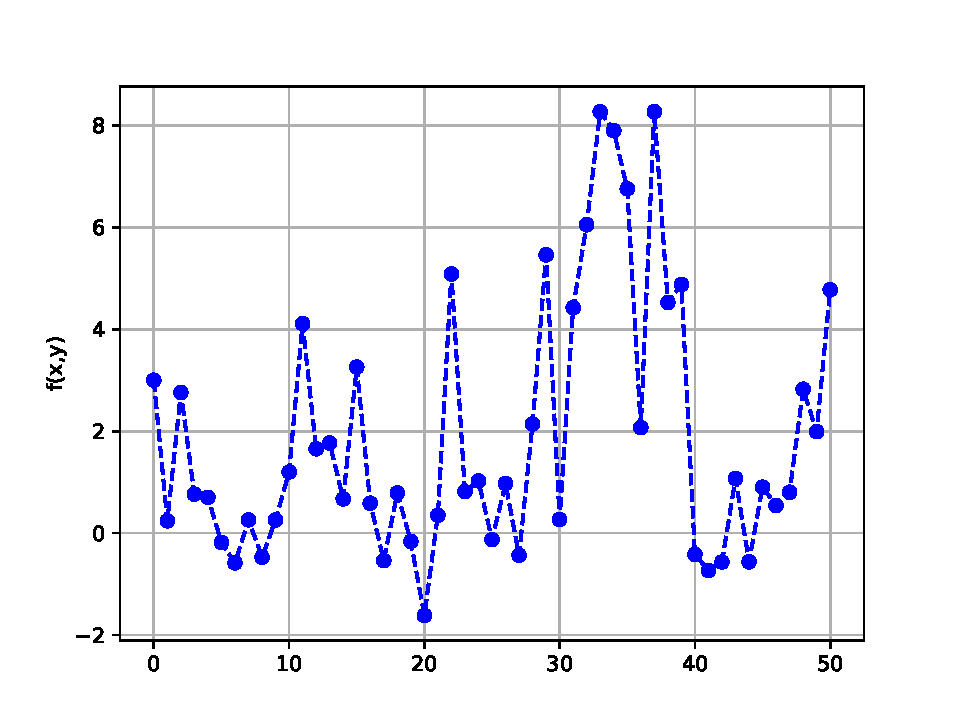
\includegraphics[scale=0.6]{media/f_evolution_e1-2-01.pdf}
  \caption{Valor de $f(x,y)$ en cada iteración con $\eta = 0.1$.}
\end{figure}

Vamos a ver qué ocurre cuando tomamos varios puntos diferentes y ejecutamos el algoritmo con $\eta = 0.01$, para tratar de que los saltos de dirección no sean muy grandes. Vamos a generar una tabla con el mínimo obtenido de cada uno de los siguientes puntos:
$(-0.5,-0.5),(1,1),(2.1,-2.1),(-3,3),(-2,2)$ y veamos qué valores alcanzan desde cada uno como mínimos locales.

\begin{table}[H]
  \begin{tabular}{llll}
  Punto inicial   & Mínimo $(x,y)$ encontrado       & Imagen en el mínimo $f(x,y)$ & Iteraciones \\
  {[}-0.5  0.5{]} & {[}-0.78365509  0.81314011{]} & 2.4931912832664618           & 50          \\
  {[}1. 1.{]}     & {[}0.67743878 1.29046913{]}   & 6.4375695988659185           & 50          \\
  {[} 2.1 -2.1{]} & {[} 0.14880583 -0.0960677 {]} & 12.490971442685037           & 50          \\
  {[}-3.  3.{]}   & {[}-2.73093565  2.71327913{]} & -0.38124949743809955         & 50          \\
  {[}-2.  2.{]}   & {[}-2.  2.{]}                 & -4.799231304517944e-31       & 50         
  \end{tabular}
\end{table}


Como vemos, cada mínimo es diferente según el punto de inicio. Esto es debido a que el mínimo local encontrado depende del punto inicial. Podemos ver los diferentes mínimos encontrados en la siguiente imagen generada:

\begin{figure}[H]
  \centering
  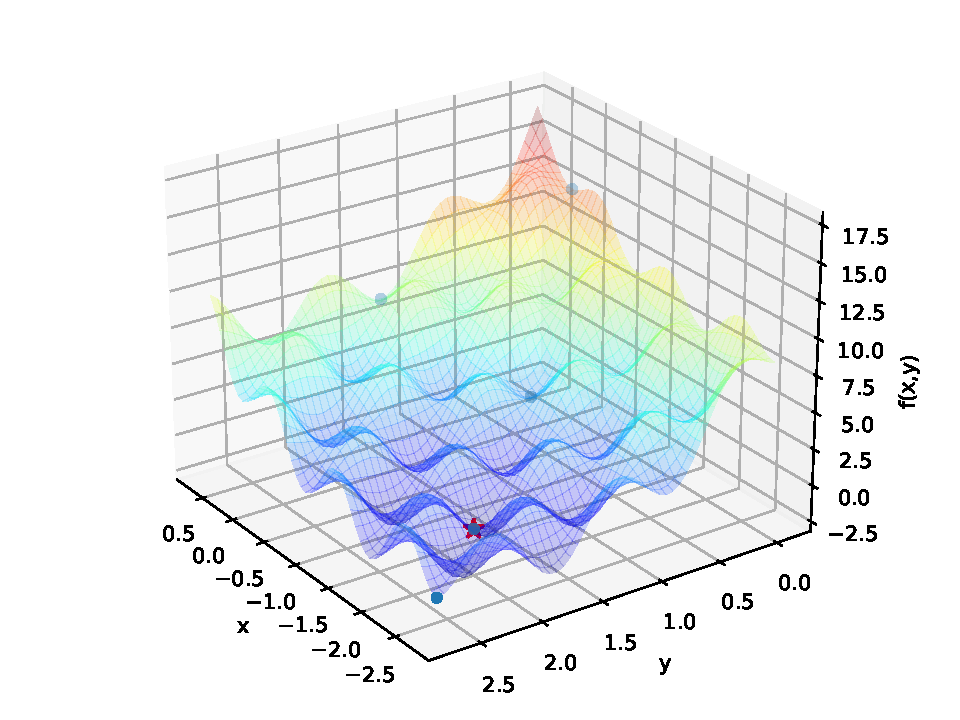
\includegraphics[scale=0.6]{media/E1-2-minimums-moved.pdf}
  \caption{Dependencia del punto inicial en el algoritmo de descenso según el gradiente.}
\end{figure}


Como se puede observar, el algoritmo está encontrando mínimos locales, que según el punto en el que hayamos iniciado son diferentes, lo cual nos muestra esta dependencia fuerte del del punto inicial que se utilice para comenzar el algoritmo, ya que el algoritmo
como sabemos acaba encontrando mínimos locales.


\subsection*{Conclusiones}

Terminamos el ejercicio haciendo una pequeña conclusión sobre los resultados obtenidos. Usando la función $f(x,y)$ definida en \eqref{eq:f} , nos ha permitido ver como partiendo desde un mismo punto y usando diferentes tasas de aprendizaje $\eta$, los mínimos que se obtienen
pueden ser radicalmente distintos. Esto es debido a que el cambio que hacemos en el punto depende de esta tasa de aprendizaje y si esta crece, el salto que da el punto en cada iteración puede hacer que el algoritmo vaya \emph{saltando} entre diferentes mínimos locales.

Además de eso, hay que comentar que el punto inicial es también muy relevante en la búsqueda del mínimo global, pues dependiendo de dónde comencemos, podemos quedarnos atrapados en un mínimo local y que nuestro algoritmo no encuente el mínimo global. Aunque ya hemos visto un ejemplo claro
con la función $f(x,y)$, podemos ver un ejemplo mucho más sencillo de que esto puede pasar incluso con funciones $f:\mathbb R \to  \mathbb R$, como en el siguiente ejemplo:

\begin{figure}[H]
\centering
\begin{tikzpicture}[scale=0.8]

  \definecolor{xdxdff}{rgb}{0.49019607843137253,0.49019607843137253,1}
  \draw[step=1cm,gray,very thin] (-1.99,-0.5) grid (3.99,0.5);
  
\draw [fill=xdxdff] (-1,0) circle (2.5pt);
\draw[color=xdxdff] (-1.3,-0.3) node {$A$};
\draw [fill=xdxdff] (3,0) circle (2.5pt);
\draw[color=xdxdff] (3.3,-0.3) node {$B$};
  \draw[scale=1, domain=-1.1:3.2, smooth, variable=\x, red] plot ({\x}, {(\x)^(4) - 5*(\x)^(3) + 5*(\x)^(2) +5*(\x) -6 });
\end{tikzpicture}
\caption{Dos mínimos locales en $f(x) = x^4 - 5 x^3 + 5 x^2 + 5 x - 6 $}
\end{figure}

Vemos que tenemos dos mínimos locales y uno de ellos es global, pero si nuestro $\eta$ no es suficientemente grande, empezando por los puntos marcados $A$ y $B$, podríamos obtener como puntos mínimos dos diferentes y en este caso uno sería el correcto (al que llegamos desde $A$) y el otro no.

Por estos dos motivos principales, concluimos que la verdadera dificultad de encontrar el mínimo global está en encontrar un punto inicial adecuado así como una tasa de aprendizaje que no sea ni demasiado grande y nos haga salirnos de esos mínimos, ni demasiado pequeña y nos fuerce
a realizar un número de iteraciones muy grande para encontrar ese mínimo global.

\newpage 

\section*{Ejercicio 2}

En esta sección, trataremos de ajustar modelos de regresión a vectores de características. La clase de funciones candidatas que utilizaremos para nuestros vectores de características es la siguiente:
$$
\mathcal H = \left\{ h : \mathbb R^{d+1} \to \mathbb R \ | \ h(x)= w^T x, \ w \in \mathbb R^{d+1}\right\}.
$$
Nuestro objetivo será encontrar este $w^T \in \mathbb R^{d+1}$. 


Trataremos con un caso en el que ajustaremos modelos a dos características
de imágenes de dígitos escritos mano. Como se indica en el enunciado, se tomará como características el \emph{nivel medio de gris} y la \emph{simetría respecto del eje vertical} y se tomarán imágenes de los
números $1$ y $5$. Vamos a comentar primero los algoritmos que vamos a utilizar para estimar los modelos de regresión.\\ 


El primero que comentaremos será el algoritmo de la \textbf{pseudoinversa}. Si dada una hipótesis $h \in \mathcal H$ lineal (esto es, $h(x) = w^T x$), consideramos la forma matricial del error en la muestra:
$$
E_{in}(w) = \frac{1}{N} \left(  w^T X^T X w - 2w^T X^T y + y^T y\right),
$$
debemos encontrar el $w$ que hace mínimo a esta expresión. Esta función es diferenciable, por lo que si calculamos su gradiente obtenemos lo siguiente:
$$
\nabla E_{in}(w) = \frac{2}{N} \left( X^T X w - X^T y\right) = \frac{2}{N} X^T \left(  X w -  y\right).
$$
Igualando a cero y suponiendo que $X^T X$ es invertible, nos queda que el mínimo $w$ es el siguiente:
$$
w = \left(X^T X\right)^{-1} X^T y = X^\dagger y, \quad \text{ donde } \quad X^\dagger = \left(X^T X\right)^{-1} X^T.
$$
Es importante remarcar que este algoritmo nos garantiza el modelo de regresión con menor error para nuestro conjunto de datos $\mathcal D$. 

El código de esta función es muy sencillo, basta con la siguiente función:
\begin{lstlisting}[language=Python]
def pseudoinverse(x,y):
	return np.linalg.inv(x.T.dot(x)).dot(x.T).dot(y)
\end{lstlisting}

Esta forma de calcular el vector de pesos $w$ mediante la pseudoinversa podría no resultar muy práctica en casos en los que nuestro conjunto de datos es mucho mayor, pues calcular la inversa de una matriz puede ser un proceso computacionalmente
muy costoso. Normalmente, para agilizar este proceso, se calcularía la descomposición \emph{SVD} de la matriz. 
Sin embargo, lo utilizaremos en esta práctica pues el tiempo de ejecución en los experimentos han sido casi inmediatos, por lo que finalmente se ha optado por dejar esta implementación.\\

Continuamos presentando el segundo algoritmo que utilizaremos. Este es el \textbf{descenso de gradiente estocástico}. Este tiene que ver con el descenso de gradiente que hemos tratado en el ejercicio anterior. La base del algoritmo
es la misma, las diferencias que los distinguen son:
\begin{itemize}
  \item Mientras que en el descenso de gradiente usábamos un \underline{único} punto (en general, suelen ser todos los datos) para evaluar el gradiente en ese punto, en el descenso de gradiente estocástico usamos un \emph{batch} (subconjunto del conjunto total de los datos) de tamaño \lstinline{batch_size} para evaluar el gradiente de la función de
  error que queremos minimizar y escoger usando este conjunto de puntos la dirección en la que nos moveremos buscando el mínimo.
  \item El criterio de parada será un número de iteraciones concreto. En este caso, consideraremos como iteración una actualización de los pesos $w$, es decir, una evaluación del gradiente en un batch.
  \item Se establece por enunciado que el punto de inicio siempre será un vector de ceros, no se le pasará como parámetro a la función como en el primer ejercicio.
\end{itemize}

Además de esto, hay que comentar sobre la función cómo se escogen los batches en cada iteración. Antes de la primera iteración, se crea un conjunto de índices del mismo tamaño que el total del conjunto de datos y se barajan los índices y se introducen en un vector. En cada iteración,
se toman los siguientes $n = batch\_size$ elementos de ese vector para la evaluación. Además, en cada iteración se comprueba si quedan elementos suficientes para obtener un batch completo en la siguiente iteración y, si no quedan suficientes, se vuelve a barajar el conjunto de índices y se empiezan
a tomar desde el primero de nuevo. Los parámetros por tanto de la función son:
\begin{enumerate}
  \item $x$ el conjunto de datos.
  \item $y$ las etiquetas de los datos.
  \item $\eta$ la tasa de aprendizaje. Se fijará a $0.1$ para los experimentos.
  \item $max\_iterations$ el número de iteraciones que se pretenden hacer.
  \item $batch\_size$, el tamaño de batch que se quiere utilizar. Lo establecemos en $32$ para este trabajo.
\end{enumerate}

Dicho esto, el código final de la función es el siguiente:
\begin{lstlisting}[language=python]
  def sgd(x,y,eta=0.01,max_iterations = 500,batch_size = 32):

	  # Initialize w
	  w = np.zeros((x.shape[1],))

	  # Create the index for selecting the batches
	  index = np.random.permutation(np.arange(len(x)))
	  current_index_pos = 0

	  for i in range(max_iterations):

	  	# Select the index that will be used
	  	iteration_index = index[current_index_pos : current_index_pos + batch_size]
	  	current_index_pos += batch_size

	  	# Update w
	  	w = w - eta*dMSE(x[iteration_index, :], y[iteration_index],w)

	  	# Re-do the index if we have used all the data
	  	if current_index_pos > len(x) or current_index_pos + batch_size > len(x):
	  		index = np.random.permutation(np.arange(len(x)))
	  		current_index_pos = 0

	return w
\end{lstlisting}

En esta función, podemos ver mencionado \lstinline{dMSE}. Esto se refiere la derivada del \textbf{error cuadrático medio }(MSE, de \emph{mean squared error}). 
El error cuadrático medio se define como
$$
MSE = E\left[(Xw - y)^2\right] =\frac{1}{N} \sum_{i=1}^N \left(X_i w_i - y_i\right)^2.
$$
como es diferenciable, podemos calcular su derivada y obtenemos:
$$
\frac{\partial MSE(w)}{\partial w_j} = \frac{2}{N} \sum_{i = 1 }^N  x_{ij}(X_i w_i - y_i).
$$

La implementación de ambas funciones es muy sencilla:
\begin{lstlisting}[language=python]
def MSE(x,y,w):
	return (np.linalg.norm(x.dot(w) - y)**2)/len(x)
def dMSE(x,y,w):
	return 2*(x.T.dot(x.dot(w) - y))/len(x)
\end{lstlisting}

Hemos presentado los algoritmos que utilizaremos y la función de error. Podemos pasar a la realización de los diferentes experimentos. Todas las representaciones están realizadas con la función \lstinline{scatter}. Esta recibe como parámetros principales:
\begin{enumerate}
\item $x$, los datos.
\item $y$, las etiquetas.
\item $ws$, un vector de vectores de pesos para dibujar los ajustes de regresión (opcional).
\item $labels$, los títulos que tendrán en el gráfico los ajustes de regresión (opcional).
\end{enumerate}
Se le pueden además indicar más parámetros para que el gráfico generado tenga más información, como los títulos de los ejes o el título del gráfico. Se puede consultar la implementación en el archivo de la práctica. Probamos la función representando los datos con los 
que trabajaremos en la primera parte de este ejercicio: 
\begin{figure}[H]
  \centering
  \includegraphics[scale=0.6]{media/"Dibujo de los datos con etiquetas".pdf}
  \caption{Datos del conjunto train con etiquetas sobre los que se realizará regresión.}
\end{figure}

Vamos a usar el gradiente descendente estocástico para estimar un modelo lineal a partir de estos datos. 
Si ejecutamos este algoritmo para nuestros datos,  obtenemos la siguiente salida:
\begin{lstlisting}[language=bash]
  Bondad del resultado para grad. descendente estocastico en 2000 iteraciones:
      Ein:  0.0814537875414063
      Eout:  0.13517885559652956
      Pesos obtenidos: [-1.23831589 -0.22450882 -0.46137888]
\end{lstlisting}
Como podemos ver, son errores bajos para el modelo lineal. Esto puede indicar que los datos son razonablemente separables y que vamos a obtener una recta de regresión que clasifique razonablemente bien nuestros datos. 
Veamos la recta de regresión que hemos obtenido mediante esta regresión, que viene dada por la expresión $w^T x = 0$:
\begin{figure}[H]
  \centering
  \includegraphics[scale=0.45]{media/"Regresión SGD en train".pdf}
  \includegraphics[scale=0.45]{media/"Regresión SGD en test".pdf}
  \caption{Resultado de la recta de regresión obtenida por SGD sobre los conjuntos de train y test.}
\end{figure}
Se puede apreciar como, efectivamente, prácticamente todos los puntos quedan bien separados en ambos conjuntos por las rectas de regresión
obtenidas.\\

Pasamos a hacer lo propio con el algoritmo de pseudoinversa. Si ejecutamos nuestra función comentada anteriormente con los datos, los resultados que obtenemos son:
\begin{lstlisting}[language=bash]
Bondad del resultado para pseudoinversa:
        Ein:  0.07918658628900395
        Eout:  0.13095383720052572
        Pesos obtenidos: [-1.11588016 -1.24859546 -0.49753165]
\end{lstlisting}
De nuevo, vemos como obtenemos errores bastante pequeños, y si dibujamos la recta obtenida en los conjuntos de entrenamiento y de prueba, obtenemos los siguientes gráficos:
\begin{figure}[H]
  \centering
  \includegraphics[scale=0.45]{media/"Regresión pseudoinversa en train".pdf}
  \includegraphics[scale=0.45]{media/"Regresión pseudoinversa en test".pdf}
  \caption{Resultado de la recta de regresión obtenida por el algoritmo de pseudoinversa sobre los conjuntos de train y test.}
\end{figure}
Al igual que en el caso anterior, prácticamente todos los puntos quedan bien separados.\\

Ahora, trataremos de comparar ambos métodos. Vemos primero que si dibujamos ambas rectas sobre el mismo gráfico, obtenemos lo siguiente:
\begin{figure}[H]
  \centering
  \includegraphics[scale=0.45]{media/"Ambas regresiones en train".pdf}
  \includegraphics[scale=0.45]{media/"Ambas regresiones en test".pdf}
  \caption{Resultado de la recta de regresión obtenida por ambos algoritmos en ambos conjuntos.}
\end{figure}

Se puede comprobar que la diferencia entre las rectas es muy pequeña, por lo que los errores también deben ser muy parecidos. Vamos a ver esto en una tabla:


\begin{table}[H]
  \centering
  \begin{tabular}{llll}
  \hline
  Algoritmo     & $E_{in}$    & $E_{out}$  & $w$ \\ \hline
  SGD           & $0.08145$ & $0.13517$ &  $(-1.238315, -0.224508, -0.461378)$ \\
  Pseudoinversa & $0.07918$ & $0.13095$ & $(-1.115880, -1.248595, -0.497531)$
  \end{tabular}
  \end{table}
Se puede observar que los errores son bastante similares en ambos casos, siendo la pseudoinversa algo menor tanto en la muestra como fuera de ella, lo cual es el resultado esperado, pues como hemos dicho, la pseudoinversa calculamos
el mínimo teórico. Vemos que los vectores de pesos $w$ que obtenemos en ambos casos son prácticamente iguales, lo cual justifica que las rectas en el dibujo sean poco dispares. Además, que el error fuera de la muestra, $E_{out}$ sea mayor que dentro de la muestra es también esperado, 
pues el error siempre puede aumentar al utilizar nuestros pesos sobre puntos desconocidos. De hecho, sabemos que en el caso lineal se tiene
$$
E_{out} = E_{in} + \mathcal O\left( \frac{d}{N}\right).
$$

Como conclusión, podríamos decir que para estos datos sería más óptimo usar la pseudoinversa aunque ambos ajustes sean prácticamente igual de buenos y que para conjuntos de datos de mayor tamaño, sería
conveniente realizar una implementación más eficiente del algoritmo de pseudoinversa.

\subsection*{Apartado 2}

Vamos a cambiar ahora los datos que vamos a utilizar y a explorar cómo cambian los errores tanto en la muestra como fuera de ella cuando cambiamos la complejidad del modelo utilizado. En este caso, los datos
se generarán utilizando la función proporcionada \lstinline{simula_unif(N,d,size)} que genera datos de forma uniforme en el conjunto $\mathcal = [-1,1]\times [-1,1]$. Si la ejecutamos y seguimos usando la misma función
\lstinline{scatter} , obtenemos lo siguiente:
\begin{figure}[H]
  \centering
  \includegraphics[scale=0.6]{media/"1000 datos generados".pdf}
  \caption{Datos generados por \emph{simula\_unif(1000,2,1.0)}.}
\end{figure}
Consideramos ahora la función $f:\mathbb R^2 \to \{-1,1\}$ dada por:
$$
f(x_1,x_2) = sign((x_1 - 0.2)^2 + x_2^2 - 0.6).
$$
Utilizamos esta función para asignar a cada punto generado por \emph{simula\_unif} una etiqueta que será 1 o -1. La implementación en python es la siguiente:

\begin{lstlisting}[language=Python]
@to_numpy
def f(x1, x2):
	return sign((x1-0.2)**2 + x2**2 - 0.6)
\end{lstlisting}


Además, introduciremos ruido en las etiquetas obtenidas, cambiando de signo el $10\%$ de la muestra. Para ello, generamos 100 índices aleatorios según el tamaño de la muestra y le cambiamos
el signo a las posiciones de estos índices. Lo comentado hasta ahora se hace en la función \lstinline{generate_data}, cuyo código es bastante sencillo:

\begin{lstlisting}[language=Python]
  def generate_data(noise = True):
	  x = simula_unif(N,dimensions,size)
	  ## Generate tags
	  y = np.array([f(a) for a in x])
	  if noise:
		  idxs = np.random.choice(N, int(0.1 * N), replace = False)
		  y[idxs] = -y[idxs]
	
	  # Homogenize
	  x = np.hstack((np.ones((1000, 1)), x))
	  return x, y

# Generamos los datos
x,y = generate_data()
\end{lstlisting}

Como podemos ver, añadimos al conjunto de datos un $1$ en la primera columna, homogenizándolo para poder usar las funciones que habíamos definido para la primera parte de la práctica. Una vez hemos
ejecutado esta generación de datos, podemos dibujarla usando \lstinline{scatter(x,y)} y obtenemos el siguiente gráfico:
\begin{figure}[H]
  \centering
  \includegraphics[scale=0.6]{media/"1000 datos generados, con etiquetas y ruido".pdf}
  \caption{Datos con etiquetas generados pot \lstinline{generate_data()}.}
\end{figure}

A simple vista, podemos observar que posiblemente una recta no sea lo más adecuado para tratar de separar nuestros datos. Vamos a comprobarlo.
Aplicamos sencillamente \lstinline{w = sgd(x,y)} para ejecutar SGD sobre nuestra población, y el resultado que obtenemos es el siguiente:

\begin{lstlisting}[language=bash]
Ejecución simple. Ajuste de modelo lineal sobre los datos.
Bondad del resultado para grad. descendente estocastico en 2000 iteraciones:
    Ein:  0.9216745788796801
\end{lstlisting}

Como vemos, el error en la muestra es muy alto en comparación con los casos anteriores. De hecho, si dibujamos con los pesos obtenidos la recta que teóricamente trata de separar los datos, el resultado es el siguiente:
\begin{figure}[H]
  \centering
  \includegraphics[scale=0.6]{media/"Regresión SGD en train en datos aleatorios".pdf}
  \caption{Regresión SGD en train en datos aleatorios.}
\end{figure}

El error fuera de la muestra $E_{out}$ será de similar calibre, ya que si generásemos otra población para que hiciese de población de test y calculásemos el error sobre ella, el resultado de que la recta que vemos separase los datos
sería muy similar. Esto vamos a verlo en lo siguiente que haremos, que será repetir este experimento $N =1000$ veces y hacer la media de los errores tanto dentro como fuera de la muestra. Para ello, creamos la función \lstinline{experiment(iterations = 1000, more_features = False)}. 
El parámetro \lstinline{more_features} será usado en el siguiente apartado. En esta función, se repetirá el experimento tantas veces como se le indique y en cada iteración, se generará un nuevo conjunto de train, un nuevo conjunto de test, se aplicará
el algoritmo SGD sobre el conjunto de train y se evaluará sobre ambos conjuntos. Se devolverá el error medio tanto dentro como fuera de la muestra. El resultado obtenido por consola es el siguiente:

\begin{lstlisting}[language=bash]
Ejecución de N=1000 experimentos de ajuste de modelo lineal en curso ...

Bondad media del resultado en 1000 experimentos para SGD con 3 características
         Average Ein:  0.9270613282456569
         Average Eout:  0.9325317891645661

\end{lstlisting}
Como intuíamos que ocurriría, el error es muy alto tanto dentro como fuera de la muestra en un conjunto grande de experimentos. Esto nos indica que regresión lineal con 3 características no es un 
buen modelo para tratar de ajustar nuestro conjunto de datos. \\

Como \textbf{valoración}, podemos decir que el ajuste con este modelo lineal no es adecuado para estos datos, ya que obtenemos unas tasas de error muy altas y necesitaríamos buscar modelos que nos permitan
ajustar nuestros datos mejor y obtener así un porcentaje de error más bajo en la clasificación. Esto es lo que haremos en el siguiente experimento.\\

El vector actual de características que tenemos es de la forma $(1,x_1,x_2)$. Consideremos ahora  la función $\phi : \mathbb R^3 \to \mathbb R^6$ dada por:
$$
\phi(1,x_1,x_2) = (1,x_1,x_2,x_1x_2,x_1^2,x_2^2).
$$
Lo que haremos ahora será, una vez generados los datos con la función anterior, llamar a la siguiente función:

\begin{lstlisting}[language=Python]
  def generate_features(x):
	  x1x2 =  np.multiply(x[:,1],x[:,2])[:, None]
	  x1x1 =  np.multiply(x[:,1],x[:,1])[:, None]
	  x2x2 =  np.multiply(x[:,2],x[:,2])[:, None]
	  return np.hstack((x, x1x2, x1x1, x2x2))

  # Creamos la población
  x = generate_data()
  # Expandimos las características de todos los puntos de la muestra
  x = generate_features(x)
\end{lstlisting}

Ahora, podemos tratar de ajustar una cónica en el plano en lugar de una recta. Si ejecutamos SGD sobre estos datos y dibujamos de nuevo la cónica que viene dada por $w^t x = 0$, obtenemos 


\begin{lstlisting}[language=bash]
Ajuste de los datos usando un modelo no lineal
Bondad del resultado en modelo de 6 características para grad. descendente estocastico en 2000 iteraciones:

        Ein:  0.5685870579996709
\end{lstlisting}

Se comprueba como el error desciende considerablemente. Vamos a dibujar la cónica obtenida para ver cómo ajusta esta a los datos:
\begin{figure}[H]
  
  \centering
  \includegraphics[scale=0.6]{media/"Regresión SGD usando modelo no lineal".pdf}
  \caption{Regresión SGD usando modelo no lineal.}
  \label{fig:no-lin}
\end{figure}

De hecho, vamos a realizar lo mismo que en el caso de una recta y vamos a repetir el experimento $N=1000$ veces y a calcular los errores $E_{in}, E_{out}$ promedios para ver qué resultado obtenemos. Esto se realiza
con la misma función \lstinline{experiment(more_features = True)}, en este caso indicando que queremos que se generen el resto de características. El resultado es el siguiente:

\begin{lstlisting}[language=bash]
Ejecucion de N=1000 experimentos de ajuste de modelo no lineal en curso ...

Bondad media del resultado en 1000 experimentos para SGD con 6 características
         Average Ein:  0.580916690228773
         Average Eout:  0.5877043117916749
\end{lstlisting}

Como podemos ver, obtenemos en media errores más bajos tanto dentro como fuera de la muestra, lo cual nos está indicando que este tipo de ajuste con características no lineales
es mejor que el que hemos hecho anteriormente con características lineales. Aún así, el error no es capaz de descender a niveles tan pequeños como los del ejercicio anterior ya que
hemos introducido una cantidad considerable de ruido, como podemos ver en la figura \ref{fig:no-lin}.

Como \textbf{conclusión} a este ejercicio, podemos decir que en este caso utilizar modelos lineales no es adecuado y es mejor aumentar la complejidad del modelo para conseguir que se reduzcan 
los errores tanto dentro como fuera de la muestra, consiguiendo así una función más parecida a la función real que se usa para etiquetar, salvo por supuesto el ruido que estamos introduciendo manualmente.

\newpage

\section*{Bonus: Método de Newton}

En este último apartado, se realizará la implementación del método de Newton. Este método nos da , dada una función $f: \mathbb R^n \to \mathbb R$, aproximaciones a los ceros de esta función. Así, si consideramos la función $\nabla f$, y tratamos de encontrar
los ceros de esta función, estaremos encontrando extremos de nuestra función $f$ (que sabemos que suele ser una función de error), y podremos encontrar entonces los mínimos deseados. Sabemos que la búsqueda de los puntos en el método de Newton se hace tomando el punto $x_{k+1}$ como:
$$
x_{k+1} = x_k - \frac{f'(x_k)}{f''(x_k)}.
$$
En nuestro caso, $f''(x_k) = \nabla^2 f(x_k) = H_f(x_k)$ pues nuestra función parte de $\mathbb R^d$, donde $H$ es la matriz Hessiana de $f$. La matriz Hessiana de $f: \mathbb R^2 \to \mathbb R$ (hablamos en este caso pues es el que usaremos en nuestro problema), viene dada por la expresión:
$$
H = \begin{pmatrix}
  \frac{\partial^2 f}{\partial^2 x^2} & \frac{\partial^2 f}{\partial x \partial y}\\
  \frac{\partial^2 f}{\partial y \partial x} & \frac{\partial^2 f}{\partial^2 y^2}
  \end{pmatrix}.
$$

Utilizando esta matriz en nuestro problema, obtenemos que en cada iteración, debemos actualizar los pesos de la siguiente manera:
$$
\Delta w = w_{k+1} - w_{k} = - H^{-1}\nabla f(w_k) \implies w_{k+1} = w_k - H^{-1}\nabla f(w_k).
$$

Recordamos que la función que teníamos en el apartado 3 del ejercicio 1 era:
$$
f(x,y) = (x+2)^2 + 2(y-2)^2 + 2\sin(2\pi x) \sin(2\pi y).
$$
Tenemos que calcular su Hessiana para poder aplicar el algoritmo. La hessiana es la siguiente:
$$
H = \begin{pmatrix} 2- 8 \pi^2 \sin(2 \pi y) \sin(2 \pi x) & 8 \pi^2 \cos(2 \pi x) \cos(2 \pi y) \\
     8 \pi^2 \cos(2 \pi x) \cos(2 \pi y) & 4- 8 \pi^2 \sin(2 \pi x) \sin(2 \pi y) 
    \end{pmatrix}.
$$

La implementación de esta hessiana es la siguiente:

\begin{lstlisting}[language=Python]
def hfxx(x, y):
  """Two times partial derivative respect x of f(x, y)."""
  return 2 - 8 * np.pi ** 2 * np.sin(2 * np.pi * y) * np.sin(2 * np.pi * x)

def hfyy(x, y):
  """Two times partial derivative respect x of f(x, y)."""
  return 4 - 8 * np.pi ** 2 * np.sin(2 * np.pi * x) * np.sin(2 * np.pi * y)

def hfxy(x, y):
  """Partial derivative respect x and then respect y of f(x,y)."""
  return 8 * np.pi ** 2 * np.cos(2 * np.pi * y) * np.cos(2 * np.pi * x)

@to_numpy
def hf(x, y):
  """f(x, y) Hessian."""
  return np.array([[hfxx(x, y), hfxy(x, y)],
        [hfxy(x, y), hfyy(x, y)]])
\end{lstlisting}
Una vez tenemos este código, podemos directamente escribir el código del método de Newton, que es tan sencillo como el de descenso del gradiente. El código resultante es el siguiente:


\begin{lstlisting}[language=Python]
  def newton(eta,dfun,hfun,maxIter,initial_point):
	  w = initial_point.copy()
	  all_w = [w]
	  for i in range(maxIter):
		  w = w - eta*np.linalg.inv(hfun(w)).dot(dfun(w))
		  all_w.append(w)
  return np.array(all_w),w
\end{lstlisting}
Como vemos, el esqueleto es igual que el del descenso de gradiente, solo que cambiamos como hemos indicado la forma de actualizar los pesos en cada iteración. Vamos ahora a realizar los experimentos que se pedían 
para el apartado 3, pero usando como método el que acabamos de explicar. Para representar los datos, se ha programado por comodidad una nueva función \lstinline{print_output_bonus} que muestra por cada ejecución del método
de Newton los parámetros con los que se ha ejecutado y el resultado obtenido. También se ha programado una función \lstinline{plot_bonus_comparison} que muestra los valores que va tomando la función $f(x,y)$ en los puntos que se le indiquen,
que serán siempre los que nos devuelva el método de Newton.\\

Comenzamos realizando el experimento que usa como punto inicial $(-1,1)$, tasa de aprendizaje $\eta = 0.01$ y un máximo de $50$ iteraciones. La consola nos indica que las coordenadas que se han alcanzado en estas 50 iteraciones son 
$$
(x,y) = ( -0.9793498 ,  0.9893767 ) \quad \text { con } \quad f(x,y) = 3.067185951
$$

Volviendo atrás en el documento, podríamos ver cómo el valor que alcanzaba el descenso de gradiente para estos mismos parámetros era de $-0.3812$, lo cual puede decirnos que el descenso de gradiente encuentra mejores mínimos para esta función y este punto inicial.

Vamos a ver cómo ha ido evolucionando la $f$ según las iteraciones del experimento:
\begin{figure}[H]
  \centering
  \includegraphics[scale=0.6]{media/"Newton's first execution, eta = 0.01".pdf}
  \caption{Ejecución del método de Newton desde el punto $(-1,1)$ con $\eta = 0.01$.}
\end{figure}

En este caso, el valor de $f$ en vez de descender ha ascendido, aunque vemos en el eje $y$ que el ascenso ha sido ínfimo. Esto podría decirnos de primeras que este algoritmo en general puede ser peor que el descenso de gradiente para esta función $f$, pero haremos una comparación más adelante. 
Ahora, nos ocupamos de hacer un nuevo experimento , en el que haremos que la tasa de aprendizaje sea $\eta = 0.1$. Si lo ejecutamos, obtenemos que las coordenadas tras las $50$ iteraciones son 
$$
(x,y) = ( -0.94632740 ,  0.97170823 ) \quad \text{ con } \quad f(x,y) =3.107976722. 
$$
Comparando con el caso anterior, tenemos una distancia entre los valores de $f$ en ambos puntos que puede no parecer muy grande, pero si observamos cómo ha ido evolucionando nuestra función $f$ en ambos casos, el gráfico que obtenemos es el siguiente:
\begin{figure}[H]
  \centering
  \includegraphics[scale=0.6]{media/"Comparison Newton's method different etas".pdf}
  \caption{Comparación de ejecución de método de Newton con $\eta =0.01$ y $\eta = 0.1$.}
\end{figure}
Vemos como el caso del $\eta$ más grande alcanza un valor de $\sim 3.10$ mucho más pronto, posiblemente debido a ese impulso que le da la tasa de aprendizaje teniendo un valor mayor. Aún así, se estabiliza en ese valor para las siguientes iteraciones mientras que con la tasa de aprendizaje $\eta = 0.01$ nunca deja de ascender, lo que podría indicar que si hiciésemos
el número de iteraciones más grande, quizá se podría alcanzar este mismo punto.\\

Estamos viendo por tanto que, al igual que en el caso del descenso de gradiente, la tasa de aprendizaje juega un papel importante a la hora de encontrar un mínimo usando el método de Newton y que es importante por tanto encontrar una tasa de aprendizaje que se adecúe a nuestro problema para no obtener tiempos de cómputo muy elevados.

Comparemos ahora qué resultados tiene el gradiente descendente con $\eta =0.01$ desde el mismo punto de inicio y en el mismo número de iteraciones con los casos anteriores:
\begin{figure}[H]
  \centering
  \includegraphics[scale=0.6]{media/"Comparision Newton's method with gradient descent".pdf}
  \caption{Comparativa del método de Newton con el gradiente descendente, ambos con el mismo punto de inicio.}
\end{figure}

Anteriormente habíamos mencionado que era posible que el gradiente descendente encontrase mejores mínimos para esta función usando las tasas de aprendizaje que hemos utilizado. Con este gráfico, confirmamos esta idea y podemos confirmar que para 
esta función, es más conveniente utilizar el algoritmo de descenso de gradiente para encontrar un mínimo, ya que la diferencia entre ambos algoritmos es bastante considerable en resultado, obteniendo el descenso de gradiente un resultado mucho más óptimo
en cuanto a minimización.

\subsection*{Apartado 2}
Ahora, al igual que hicimos en el ejercicio 1, vamos a ejecutar el método de Newton sobre varios puntos diferentes con la misma tasa de aprendizaje para todos y vamos a ver qué puntos se obtienen como mínimos y qué valores toma la función $f$ en cada
uno de ellos. El resultado de la ejecución es el siguiente:
\begin{table}[H]
  \begin{tabular}{llll}
  Punto inicial               & Mínimo (x,y) encontrado                & Imagen $f(x,y)$ en el mínimo                & Iteraciones \\
  {[}-0.5  0.5{]} & {[}-0.4688174   0.48387437{]} & 6.902412398443703      & 50         \\
  {[}1. 1.{]}     & {[}1.02206051 0.96894401{]}   & 11.205423036736665     & 50         \\
  {[} 2.1 -2.1{]} & {[} 2.11759899 -2.07774574{]} & 49.5785291890354       & 50         \\
  {[}-3.  3.{]}   & {[}-3.02065016  3.01062326{]} & 3.067185951548828      & 50         \\
  {[}-2.  2.{]}   & {[}-2.  2.{]}                 & -4.799231304517944e-31 & 50        
  \end{tabular}
\end{table}
Al igual que en el caso anterior, los mínimos que se encuentran según en el punto en el que empecemos son totalmente diferntes. Ahora, además, los valores de $f$ tienen incluso más distancia entre ellos, además de no parecerse mucho a los que se encuentran usando
el descenso de gradiente, salvo en el caso del punto $(-2,2)$. Esto es debido a que este punto es probablemente el mínimo local. Vamos a hacer una comparación de los valores que toma la función en los mínimos usando ambos algoritmos según el punto en el que se inicia 
la búsqueda de estos mínimos:

\begin{table}[H]
  \begin{tabular}{lll}
  Punto inicial   & f(x,y) según Descenso de Gradiente & f(x,y) según Newton     \\
  {[}-0.5  0.5{]} & 2.4931912832664618                 & 6.902412398443703                        \\
  {[}1. 1.{]}     & 6.4375695988659185                 & 11.205423036736665                       \\
  {[} 2.1 -2.1{]} & 12.490971442685037                 & 49.5785291890354                         \\
  {[}-3.  3.{]}   & -0.38124949743809955               & 3.067185951548828                        \\
  {[}-2.  2.{]}   & -4.799231304517944e-31             & -4.799231304517944e-31                   
  \end{tabular}
  \end{table}

  Como comentábamos, los mínimos que encuentra el descenso de gradiente son bastante inferiores en todos los casos, lo cual nos puede indicar que con tasas de aprendizaje $\eta$ similares y pequeñas, además de no necesariamente estar cerca del mínimo que se está buscando, este método es mucho más estable y 
  óptimo para la búsqueda de mínimos en funciones. Por último, podemos ver qué valores han ido tomando la función $f$ en cada iteración para cada uno de los puntos. Representaremos tanto el método de Newton para los puntos que se nos ha dado, como el gradiente descendente en los puntos $(1,1)$ y $(-2.1,2.1)$ (los
  cuales también son usados en el método de Newton). El resultado es el siguiente:
  \begin{figure}[H]
    \centering
    \includegraphics[scale=0.6]{media/"Starting in all points compared to GD".pdf}
    \caption{Valores de $f$ en las iteraciones desde los puntos anteriores según Newton, y desde dos puntos según el descenso de gradiente.}
  \end{figure}
  
  Como podemos observar, en el método de Newton las soluciones encontradas no suelen variar mucho y si lo hacen es de forma brusca como en el caso del punto
  de inicio $(2.1,-2.1)$. Mientras tanto, en el descenso de gradiente, nuestra función $f$ por lo general va siempre hacia valores menores de la misma.

  Es por esto que como \texbf{conclusión}, podemos decir que  para esta función es mejor utilizar el gradiente descendente pues encuentra mínimos mejores, es menos restrictiva (no requiere en general que la función sea dos veces derivable) y es más 
  fácil de calcular, pues no tenemos que calcular una inversa. Sin embargo, no podemos afirmar que esto sea así para todas las funciones, y puede que en otras que tengan menor cantidad de puntos críticos como pudimos ver que esta tiene en anteriores representaciones, el método
  de Newton sea mejor.

\end{document}
